\chapter{초대칭이 중요할 수 있는 이유}

\lectureoverview{이 장의 여러 주제는 진공 요동으로 연결된다.
경계 조건은 카시미르 힘을 만들고, 루프 효과는 힉스 질량을 위협하며, 새로운 가상 입자는 게이지 결합의 에너지에 따른 변화를 바꾸고, 진공 에너지는 우주의 팽창을 좌우한다. 이러한 문제들은 힉스 척도를 안정화하고 암흑물질 후보를 제공하며 게이지 결합의 통일을 개선하는 방법으로 저에너지 초대칭을 생각해 보게 한다. 이어서 그라스만 좌표를 사용해 초장을 구성하고, 베레진 적분으로 초대칭 작용을 구한다.}

\section{반사판 사이의 진공 요동}

카시미르 효과에 관한 질문을 먼저 정리하며 초대칭으로 돌아가 보자. 서로 \(d\)만큼 떨어진 평행한 반사판 두 개를 놓는다. 실제 입자가 하나도 없더라도 양자장은 진공 요동을 갖는다. 이를 가상 과정으로 그려 볼 수도 있고, 동등하게 장의 진동자 모드가 갖는 영점 운동으로 볼 수도 있다. 판은 경계 조건을 부과하므로, 판 사이에서 허용되는 요동은 제한 없는 공간에서의 요동과 달라진다.

중요한 것은 에너지의 절대적인 영점이 아니라 판 사이 거리가 변할 때 생기는 변화다. 단위 면적당 진공 에너지를 \(\mathcal E(d)=E(d)/A\)로 나타내자. \(\mathcal E\)가 \(d\)에 따라 달라지면 이는 퍼텐셜 에너지이며, 단위 면적당 힘은 다음과 같다.
\begin{equation}
\frac{F}{A}=-\frac{d\mathcal E}{dd}.
\end{equation}
따라서 가상 과정의 재배열은 관측 가능한 힘으로 나타난다. 이상적인 도체판을 예로 든 익숙한 전자기적 결과에서 에너지와 압력은 다음과 같다.
\begin{align}
\mathcal E(d)&=-\frac{\pi^2}{720\,d^3},\\
\frac{F}{A}&=-\frac{\pi^2}{240\,d^4},
\end{align}
단위는 \(\hbar=c=1\)이다.\editorialnote{이 계수들과 \(d^{-3}\)에 따른 면적당 에너지 및 \(d^{-4}\)에 따른 압력의 구분으로 칠판에서 제기된 차원에 관한 의문을 해소할 수 있다. 이는 여기서 유도하는 결과가 아니라, 이상적인 판에 대해 잘 알려진 표준 결과다.} 마이너스 부호는 인력을 뜻한다.

\begin{classroomqa}
\audiencequestion{네제곱에 반비례하는 것은 힘인가, 에너지인가? \lecturetimestamp{00:04:39}}
\lecturerresponse{시공간이 4차원일 때 평행판의 단위 면적당 에너지는 \(d^{-3}\)에 따라 감소하지만, \(d\)에 대해 미분하면 단위 면적당 힘은 \(d^{-4}\)에 따라 감소한다. \(\hbar\)와 \(c\)를 다시 넣으면 차원 분석만으로도 이 거듭제곱을 정할 수 있다.}
\end{classroomqa}

계산을 판이 가상 광자 루프를 끊는 과정이라고 요약하기도 한다. 이 그림은 지나치게 문자 그대로 받아들이지 않는다면 유용하다. 정확한 계산은 허용되는 장 모드의 스펙트럼 변화, 또는 동등하게 양자 유효 작용의 변화다. 어느 쪽으로 설명하든 거리 의존적인 에너지는 같다.

\begin{classroomqa}
\audiencequestion{카시미르 힘은 인력이 아니라 척력일 수도 있나요? \lecturetimestamp{00:07:48}}
\lecturerresponse{그럴 수 있다. 부호는 보편적으로 정해져 있지 않고 장, 기하학적 구조, 재료, 경계 조건에 따라 달라진다. 페르미온 루프는 보손 루프와 반대되는 루프 부호를 갖는 경우가 많아 칠판에서 나온 제안의 동기가 되지만, 페르미온 통계만으로 모든 카시미르 힘이 척력이어야 한다는 일반 정리가 성립하는 것은 아니다.\editorialnote{이 단서는 잠정적으로 제시했던 수업 중 답변을, 잘못된 보편 법칙을 피하는 데 필요한 일반적인 진술로 다듬는다.}}
\end{classroomqa}

\subsection{진공 에너지의 증거로 무엇을 들 수 있을까?}

카시미르 힘은 측정되며, 원자 관측량도 진공 루프에 민감하다. 그러나 이 사실들만으로는 진공의 절대 에너지가 중력에 기여한다는 점이 입증되지 않는다. 카시미르 실험은 경계로 인해 생기는 에너지 차이를 측정한다. 절대 영점 에너지를 발산하는 합에 조작적 의미를 부여하지 않고도 같은 힘을 설명할 수 있다.

결정적인 검증은 중력에서 나온다. 에너지는 중력 전하다. 빈 공간에 균일한 에너지 밀도가 있다면 아인슈타인 방정식에 들어가 우주의 팽창에 영향을 주어야 한다. 따라서 우주의 가속 팽창은 진공과 비슷한 성분에 대한 직접적인 중력 증거다.

\begin{classroomqa}
\audiencequestion{물리학자들이 진공 에너지가 무엇인지 모르는 것처럼, 대중 매체에서는 왜 진공 에너지를 수수께끼라고 부르나요? \lecturetimestamp{00:08:19}}
\lecturerresponse{양자장론에서는 모든 장에 영점 기여가 있으므로 진공 에너지가 존재할 가능성 자체는 수수께끼가 아니다. 수수께끼는 그 양에 있다. 알려진 양자장과 고에너지 컷오프를 바탕으로 한 추정값에 비해, 중력에 기여하는 값이 왜 그토록 극도로 작은가? 놀라운 것은 진공 에너지의 존재 자체가 아니라 그것이 거의 없다는 점이다.}
\end{classroomqa}

오랫동안 관측으로 정해진 상한은 매우 작아서, 우주상수를 정확히 영으로 놓고 상쇄를 강제하는 원리를 찾고 싶은 심리적 유혹이 있었다. 그러나 우주론 관측이 정밀해지면서 작지만 0이 아닌 값이 발견되었다. 이 발견으로 진공 에너지가 개념적으로 낯선 것이 된 것은 아니었다. 설명되지 않은 억제의 정도를 더는 외면할 수 없게 된 것이다. 관련된 비교는 가정하는 자외선 척도에 따라 달라지지만, 자연스러운 고에너지 추정은 모두 엄청난 상쇄를 요구한다.

\section{초전하 하나가 다입자 상태에 작용하면}

초대칭을 지지하는 이유를 열거하기 전에, 먼저 한 가지 역설처럼 보이는 문제를 풀어야 한다. 보손은 하나의 모드에 임의로 많은 수가 들어갈 수 있지만, 페르미온 모드의 점유수는 0 또는 1이다. 보손과 페르미온을 서로 바꾸는 대칭이 있다면, 한 모드에 있는 보손 천 개를 같은 모드에서 금지된 페르미온 천 개로 바꾸는 것일까?

아니다. 페르미온 생성자는 한 번에 양자 하나를 바꾼다. 진동자 모형에서 \(a\)가 보손을 소멸시키고 \(c^\dagger\)가 그 짝인 페르미온을 생성하게 하자. 초전하 하나는 다음과 같이 나타낼 수 있다.
\begin{equation}
Q=c^\dagger a.
\end{equation}
보손이 \(n\)개 있고 페르미온은 없는 상태에 작용시키면,
\begin{equation}
Q\ket{n,0}
=\sqrt n\,\ket{n-1,1}.
\end{equation}
보손 하나가 제거되고 페르미온 하나가 들어간다. 같은 전하를 다시 작용시키면 결과는 0이다.
\begin{equation}
Q^2=(c^\dagger)^2a^2=0.
\end{equation}
이는 페르미온 생성 연산자에서 물려받은 멱등성이다.

\begin{classroomqa}
\audiencequestion{많은 보손이 같은 상태를 차지하고 있다면, 초대칭 변환은 왜 그 상태에 있는 보손들을 다수의 페르미온으로 바꾸어 배타 원리를 위반하게 만들지 않을까? \lecturetimestamp{00:12:05}}
\lecturerresponse{생성자는 전체 점유 상태를 통째로 바꾸지 않는다. 페르미온 수를 한 단위만큼 바꾼다. 같은 페르미온 전하는 보통의 회전 생성자처럼 거듭 합성할 수 없는데, 그 제곱이 사라지기 때문이다. 이에 대응하는 전하를 작용시키면 그 교환을 되돌릴 수 있고, 혼합 반교환자는 시간 병진으로 닫힌다.}
\end{classroomqa}

마지막 문장은 핵심이다. 약식 표기 \(Q^2=0\)는 개별 카이랄 성분이나 방금 쓴 단순한 전하에 적용된다. 모든 초전하의 곱이 사라진다는 뜻은 아니다. 네 차원 초대칭에서,
\begin{equation}
\{Q_\alpha,\bar Q_{\dot\beta}\}
=2\sigma^\mu_{\alpha\dot\beta}P_\mu,
\end{equation}
한편 중심 전하가 없는 최소 대수에서는
\begin{equation}
\{Q_\alpha,Q_\beta\}=0,
\qquad
\{\bar Q_{\dot\alpha},\bar Q_{\dot\beta}\}=0
\end{equation}
가 성립한다.\editorialnote{이 성분 표현은 같은 \(Q\)를 거듭 작용시키면 사라지는 반면, 초전하와 그 켤레가 함께 병진을 생성한다는 강의실식 약식 설명을 정확히 나타낸다.}

\section{저에너지 초대칭을 탐색할 세 가지 이유}

\begin{classroomqa}
\audiencequestion{진공 에너지 상쇄 말고도 초대칭을 뒷받침하는 동기가 있나요? \lecturetimestamp{00:15:06}}
\lecturerresponse{서로 긴밀히 관련된 동기는 세 가지다. 힉스 자기 에너지의 제어, 안정한 암흑물질 입자 후보, 그리고 고에너지에서 게이지 결합이 훨씬 더 정확히 만난다는 점이다. 어느 하나도 자연계에서 초대칭이 실현된다는 것을 증명하지는 않지만, 세 가지를 함께 보면 초대칭은 진지하게 검증할 가치가 있는 이론이다.}
\end{classroomqa}

\emph{저에너지 초대칭}이라는 말은 상대적인 표현이다. 초짝입자의 질량이 일상적인 척도에서 가볍다는 뜻이 아니라, 질량이 전약 척도와 가속기 척도보다 엄청나게 높지는 않다는 뜻이다. 초짝입자의 질량이 한없이 높아지면 세 가지 논거 모두 약해진다.

\subsection{힉스 척도 보호하기}

스칼라 질량은 고에너지 물리에 유별나게 민감하다. 개략적으로 보손 루프는 다음 형태의 보정을 만든다.
\begin{equation}
\delta m_H^2\big|_{\mathrm B}
\sim +\frac{\lambda}{16\pi^2}\Lambda^2,
\end{equation}
여기서 \(\Lambda\)는 유효 이론을 적용하는 에너지 척도를 나타낸다. 페르미온 루프는 반대 부호를 갖는다.
\begin{equation}
\delta m_H^2\big|_{\mathrm F}
\sim -\frac{|y|^2}{8\pi^2}\Lambda^2.
\end{equation}
계수는 상호작용과 장의 중복도에 따라 달라지지만, 초대칭은 계수들을 서로 연관시켜 초짝 사이에서 선도 자외선 민감도가 상쇄되도록 한다.\editorialnote{이 개략적인 루프 식은 자기 에너지에 관한 정성적 논거의 바탕이 되는 수학을 보여 준다. 표준모형의 힉스 질량을 완전히 계산하려는 식은 아니다.}

힉스의 진공 기댓값이 전약 척도를 정하므로 이 점이 중요하다. 게이지 보손과 페르미온의 질량은 다음과 같은 관계를 따른다.
\begin{equation}
m_W=\frac{gv}{2},
\qquad
m_f=\frac{y_fv}{\sqrt2}.
\end{equation}
힉스 부문이 자연스럽게 엄청난 척도로 밀려난다면, 익숙한 저에너지 입자 스펙트럼은 사라질 것이다. 이를 유지하려면 복사 보정과 맨질량 매개변수를 극도로 정밀하게 맞춰야 한다.

정확한 초대칭이라면 상쇄도 정확하겠지만, 관측된 보손과 페르미온의 질량이 서로 다르므로 정확한 초대칭은 이미 배제되어 있다. 연성 깨짐 초대칭에서는 이차 민감도가 초짝 질량 분할에 대한 의존성으로 대체된다. 개략적으로
\begin{equation}
\delta m_H^2
\sim
\frac{g^2}{16\pi^2}
\left(m_{\mathrm{soft}}^2-m_{\mathrm{ordinary}}^2\right)
\ln\frac{\Lambda^2}{m_{\mathrm{soft}}^2}.
\end{equation}
질량 분할이 너무 크지 않을 때에만 상쇄가 유용하게 유지된다.

\subsection{암흑물질 붕괴 연쇄의 안정한 종착점}

스펙트럼을 보통 입자와 초짝입자로 나누어 보자. 페르미온에는 보손 초짝이 있고, 보손에는 페르미온 초짝이 있다. 두 부류를 구분하는 패리티를 상호작용이 보존한다면, 초짝입자가 붕괴할 때 다른 초짝입자가 남아야 한다.
\begin{equation}
\widetilde X
\longrightarrow X+\widetilde Y
\longrightarrow X+Y+\widetilde Z
\longrightarrow\cdots.
\end{equation}
붕괴 연쇄에서 마지막 초짝입자를 없앨 수는 없다. 따라서 연쇄는 가장 가벼운 초대칭 입자인 LSP에서 끝난다.

널리 쓰이는 대칭은 \(R\)-패리티다.
\begin{equation}
R_p=(-1)^{3(B-L)+2s}.
\end{equation}
표준모형 입자는 \(R_p=+1\)이고, 초짝입자는 \(R_p=-1\)이다. \(R_p\)가 정확히 보존되면 모든 상호작용에는 초짝입자가 짝수 개 포함되며 LSP는 안정하다.\editorialnote{초대칭만으로 안정한 LSP가 보장되지는 않는다. 안정하려면 \(R\)-패리티나 같은 결과를 낳는 다른 대칭이 보존되어야 한다. 그렇지 않으면 LSP는 붕괴할 수 있다.}

암흑물질은 우주론적 시간 척도보다 오래 살아남아야 한다. 또한 눈에 보이는 은하 원반을 반복해서 지나가도 에너지를 상당량 잃지 않을 만큼 약하게 상호작용해야 한다. 전하를 띠거나 강하게 상호작용하는 입자 집단은 산란하고 에너지를 소산하여 보통 물질과 같은 얇은 구조로 모이는 경향이 있다. 관측된 넓은 헤일로는 대신 전기적으로 중성이며 약하게 상호작용하는 성분을 시사한다.

그렇다고 LSP가 무엇인지 유일하게 정해지는 것은 아니다. 모형과 대칭 깨짐 양상에 따라 후보는 전약 게이지노와 힉시노가 섞인 중성 입자일 수도 있고, 그래비티노일 수도 있다. 전하를 띠거나 색전하를 가진 후보는 강한 제약을 받는다. 초대칭이 제공하는 것은 보장된 답이 아니라 중성이며 오래 살아남는 종착점을 만들어 내는 자연스러운 메커니즘이다.

\section{에너지에 따른 결합의 변화와 통일의 단서}

세 번째 동기는 전하 차폐에서 출발한다. 가상 입자가 상호작용을 둘러싸므로 측정되는 결합은 에너지 척도에 따라 달라진다. 전자기학에서는 광자 전파자에 삽입된 전자-양전자 루프가 먼 거리에서 전하를 차폐한다. 더 짧은 거리, 즉 더 높은 운동량 전달에서는 탐침 사이에 놓인 분극 구름의 양이 줄어 유효 전하가 커진다.

다음과 같이 쓰자.
\begin{equation}
\alpha_i=\frac{g_i^2}{4\pi}.
\end{equation}
1루프 근사에서 역결합은 에너지의 로그에 따라 선형으로 변한다.
\begin{equation}
\frac{d\alpha_i^{-1}}{d\ln\mu}
=-\frac{b_i}{2\pi}.
\end{equation}
따라서
\begin{equation}
\alpha_i^{-1}(\mu)
=\alpha_i^{-1}(\mu_0)
-\frac{b_i}{2\pi}\ln\frac{\mu}{\mu_0}.
\end{equation}
\editorialnote{이 1루프 방정식은 로그 에너지를 가로축으로 그렸을 때 거의 직선인 그래프의 정확한 표현이다. 문턱 효과와 고차 루프 보정으로 직선은 조금 휘어진다.}

전약 척도 위에서 기본 게이지 결합 세 가지는 다음 게이지 군에 해당한다.
\begin{equation}
U(1)_Y,\qquad SU(2)_L,\qquad SU(3)_c.
\end{equation}
저에너지에서 직관을 위해 사용하는 전자기 결합은 전약 대칭 깨짐 뒤 첫 번째와 두 번째 결합의 조합이다. QCD에서는 비가환 게이지장이 반차폐를 일으킨다. 이것이 짧은 거리에서 강한 결합이 약해지는 점근적 자유 현상이다. 따라서 \(\alpha_3^{-1}\)은 \(\ln\mu\)에 따라 증가하는 반면, 나머지 역결합은 기울기가 다르다.

표준모형 곡선은 서로 가까워지는 듯 보이지만 한 점에서 만나지는 않는다. 초짝입자는 가상 루프를 바꾸고, 따라서 계수 \(b_i\)를 바꾼다. 통상적인 대통일 정규화에서
\begin{align}
(b_1,b_2,b_3)_{\mathrm{SM}}
&=\left(\frac{41}{10},-\frac{19}{6},-7\right),\\
(b_1,b_2,b_3)_{\mathrm{MSSM}}
&=\left(\frac{33}{5},1,-3\right).
\end{align}
초짝입자 문턱이 TeV 척도 부근에 있으면, 외삽한 초대칭 곡선은 다음 부근에서 훨씬 정확하게 만난다.
\begin{equation}
M_{\mathrm{GUT}}\sim 10^{16}\ \mathrm{GeV}.
\end{equation}
어떤 실험도 이 척도에 직접 도달하지 못한다. 저에너지 결합을 측정하고, 장의 구성으로 에너지에 따른 변화를 정한 다음, 여러 자릿수에 걸쳐 곡선을 외삽한다. 두 직선은 언제나 어딘가에서 교차한다. 서로 독립적인 세 직선이 한 점 부근에서 만난다는 것이 의미 있는 관측이다.

\begin{classroomqa}
\audiencequestion{개선된 외삽은 정확한 초대칭과 초짝입자의 동일한 질량을 가정하나요? \lecturetimestamp{00:38:09}}
\lecturerresponse{아니다. 초대칭은 깨져 있으므로 질량에 분할이 생긴다. 중요한 것은 초짝입자 루프가 에너지에 따른 변화에 언제부터 들어오는가이다. 초짝입자가 지나치게 무겁지 않다면 세 결합의 기울기가 충분히 이른 시기에 바뀌어 서로 수렴한다. 초짝입자가 극도로 무거우면 초대칭 문턱이 너무 늦게 나타나 개선된 수렴이 사라진다.}
\end{classroomqa}

문턱 보정과 미지의 고에너지 스펙트럼 때문에 세 직선이 수학적으로 정확히 한 점에서 만난다고 단정할 수는 없다. 그래도 결과는 놀랍다. 힉스 문제를 완화하고 열적 암흑물질 후보를 제공하는 바로 그 근사적인 초짝입자 척도가 통일도 개선한다.

\subsection{중력과 공통의 고에너지 척도}

중력은 전하가 에너지 자체라는 점에서 다르게 작용한다. 질량중심 에너지 \(E\)에서 유용한 무차원 척도는 다음과 같다.
\begin{equation}
\alpha_G(E)\sim GE^2
=\left(\frac{E}{M_{\mathrm{Pl}}}\right)^2.
\end{equation}
일상적인 에너지에서는 이 값이 믿기 어려울 만큼 작지만, \(E\)의 제곱에 비례해 증가한다. 따라서 그 역수는 로그에 따라 변하는 게이지 역결합보다 훨씬 빠르게 감소하여 플랑크 척도 부근에서 1 정도가 된다.

이 비교는 모든 상호작용이 서로 가까운 높은 에너지 척도에서 지배될 가능성을 시사하지만, 게이지 통일보다는 덜 명확하다. 게이지 결합은 재규격화 가능한 장론의 무차원 매개변수인 반면, 뉴턴 상수는 차원을 가지므로 중력을 같은 그래프에 나타내려면 규약을 정해야 한다.

\begin{classroomqa}
\audiencequestion{초짝입자는 같은 세 게이지 상호작용에 참여하나요, 아니면 새로운 힘을 정의하나요? \lecturetimestamp{00:42:35}}
\lecturerresponse{초짝입자는 짝이 되는 입자와 같은 게이지 양자수를 가진다. 셀렉트론은 전자와 같은 전하를 띠고, 스쿼크는 스핀과 질량은 다르지만 해당 쿼크와 같은 색전하 및 전약 전하를 가진다. 따라서 초짝입자의 루프는 새로운 게이지 상호작용 세 가지를 도입하는 것이 아니라 기존의 같은 게이지 상호작용을 바꾼다.}
\end{classroomqa}

\begin{classroomqa}
\audiencequestion{LHC에서 초짝입자를 발견하면 초대칭의 결정적 증거가 되나요? \lecturetimestamp{00:43:27}}
\lecturerresponse{낯선 입자 하나만 발견하고 그 이름을 붙이는 것으로는 충분하지 않다. 그러나 스핀, 전하, 질량, 결합 사이의 초대칭 관계를 따르는 초짝입자 스펙트럼은 매우 뚜렷한 특징을 보일 것이다. 초대칭은 서로 연관된 여러 제약을 부과하므로, 구체적인 상호작용 양상이 결정적인 검증이 된다.}
\end{classroomqa}

\subsection{척도를 높이면 대가를 치르는 이유}

초짝입자의 질량이 실험으로 도달할 수 있는 범위를 조금 넘어서는 정도라면 세 가지 동기는 여전히 작동할 수 있다. 질량을 여러 자릿수만큼 높이면 각각의 논거가 약해진다.
\begin{enumerate}\item 힉스 질량의 상쇄 뒤에도 질량 분할에 대한 큰 잔여 민감도가 남는다.
\item 통상적인 약한 척도의 열적 잔존 입자가 예상한 척도에서 더는 생기지 않는다.
\item 게이지 결합의 에너지에 따른 변화에서 문턱이 더 높은 에너지로 밀려 세 결합의 수렴이 덜 정확해진다.
\end{enumerate}
초대칭은 훨씬 높은 척도에서 여전히 존재할 수 있지만, 그런 경우에는 이 특정한 저에너지 문제들을 그만큼 경제적인 방식으로 해결하지 못한다. 이 아이디어가 오래 이어졌다고 해서 자연이 반드시 이를 따른다는 증거가 되는 것은 아니다. 다만 결정적인 검증을 받을 만큼 일관성 있는 제안이라는 뜻이다.

\section{암흑물질에 관해 우주론으로 알 수 있는 것과 알 수 없는 것}

\begin{classroomqa}
\audiencequestion{핵합성으로 수소와 헬륨을 제한하듯, 표준 우주론으로 암흑물질의 양과 암흑물질 입자 하나의 질량을 알아낼 수 있나요? \lecturetimestamp{00:46:32}}
\lecturerresponse{우주론은 암흑물질의 총 질량 밀도를 매우 정확히 측정하지만, 밀도만으로는 질량과 개수를 구분할 수 없다. 같은 밀도를 무거운 입자 몇 개가 만들 수도 있고, 매우 가벼운 입자가 엄청나게 많이 만들어 낼 수도 있다. 미시적 입자를 규명하려면 추가 이론이나 중력 이외의 관측이 필요하다.}
\end{classroomqa}

이러한 모호함을 보여 주는 두 가지 대표적인 가능성이 있다. 전약 척도 또는 TeV 척도 부근의 약하게 상호작용하는 입자는 뜨거운 열적 열평형계에서 동결 이탈할 수 있다. 반대편 극단에서는 액시온과 같은 매우 가벼운 보손이 결맞은 장 배치나 응축 상태를 이룰 수 있다. 가장 잘 발달한 두 메커니즘이 양극단 부근에 있다고 해서 그 사이의 가능성이 금지되는 것은 아니다.

헤일로의 구조 자체도 중요한 제약을 준다. 암흑물질은 보통 물질을 거의 마찰 없이 지나가므로 빛나는 원반으로 붕괴하지 않고 공간적으로 넓게 퍼진 채 남는다. 회전 곡선과 다른 중력 현상으로 질량이 존재한다는 사실은 알 수 있지만, 그 현상만으로 입자의 개수를 셀 수는 없다.

\begin{classroomqa}
\audiencequestion{초기 우주에는 초입자만 있다가 나중에 붕괴하여 지금 보이는 입자가 되었을 수도 있나요? \lecturetimestamp{00:49:11}}
\lecturerresponse{모든 관련 질량보다 훨씬 높은 온도에서는 빠른 반응으로 종들이 임의로 한쪽에 치우친 분포가 아니라 열평형에 가까워진다. 수가 부족한 초짝입자는 보통 입자들의 충돌로 생성되고, 초짝입자들의 충돌과 붕괴는 보통 입자를 다시 보충한다. 정확한 풍부도는 상호작용과 자유도에 따라 달라지지만, 뜨거운 플라스마는 계속 균형을 이루는 쪽으로 나아간다.}
\end{classroomqa}

우주가 식으면 무거운 종의 수는 볼츠만 억제로 줄고, 이들은 소멸하거나 붕괴한다. 안정한 LSP는 상호작용률이 우주 팽창보다 느려지면 열평형 상태를 더 이상 따라가지 않는다.
\begin{equation}
\Gamma_{\mathrm{ann}}
\sim n\langle\sigma v\rangle
\lesssim H.
\end{equation}
남은 입자들이 잔존 풍부도를 이룬다.\editorialnote{이 동결 이탈 조건은 열적 균형에 관한 설명을 정량적으로 마무리해 주는 표준 결과다. 특히 상호작용이 매우 약한 그래비티노를 비롯한 다른 LSP 후보는 비열적 이력을 가질 수 있다.}

\begin{classroomqa}
\audiencequestion{LSP는 어떤 보통 입자의 초짝이며, 반드시 상호작용하지 않아야 하나요? \lecturetimestamp{00:51:05}}
\lecturerresponse{모형에 무관한 답은 없다. 암흑물질 후보가 될 만한 LSP는 전기적으로 중성이며 색전하가 없을 것으로 예상되지만, 완전히 상호작용하지 않아야 하는 것은 아니다. 광자, 약한 게이지 보손, 힉스 장과 연관된 혼합 상태일 수도 있고, 그래비티노일 수도 있다. 정확한 정체는 초대칭 깨짐 스펙트럼에 따라 정해진다.}
\end{classroomqa}

\section{진공 다이어그램, 자기 에너지 다이어그램, 그리고 팽창}

\begin{classroomqa}
\audiencequestion{힉스 발산과 진공 에너지 발산은 어떻게 다른가요? \lecturetimestamp{00:52:09}}
\lecturerresponse{진공 다이어그램에는 외부 입자선이 없다. 이 다이어그램은 빈 공간의 유효 작용을 바꾸어 진공 에너지에 기여한다. 힉스 자기 에너지 다이어그램에는 외부 힉스 다리가 두 개 있다. 이 다이어그램은 힉스 전파자를 바꾸어 질량에 영향을 준다. 둘 다 가상 요동을 포함하지만, 서로 다른 질문에 답한다.}
\end{classroomqa}

실제 입자를 진공 속에 끼워 넣은 불순물로 생각해 볼 수 있다. 이 불순물에 붙는 진공 요동은 입자의 전파와 질량을 바꾼다. 카시미르 판도 진공 요동을 바꾸지만, 거시적인 경계 조건을 통해서다. 두 경우에 공통으로 작용하는 것은 끼워 넣은 대상에 대한 양자 요동의 반응이다. 보정되는 관측량은 경우마다 다르다.

\vspace{-2pt}\subsection{물질, 복사, 진공 에너지는 서로 다르게 희석된다}

\(a(t)\)를 우주론적 척도 인자라고 하고,
\begin{equation}
H=\frac{\dot a}{a}
\end{equation}
허블 매개변수를 다음과 같이 정의하자. 균일한 우주에서 국소적인 응력-에너지 보존은 다음을 준다.
\begin{equation}
\dot\rho+3H(\rho+p)=0.
\end{equation}
상태방정식이 \(p=w\rho\)이면 이를 적분하여 다음을 얻는다.
\begin{equation}
\rho(a)\propto a^{-3(1+w)}.
\end{equation}
\editorialnote{연속 방정식은 입자 수와 파장 늘어남으로 희석을 설명하는 간결한 유도 과정을 제공한다.}

차갑고 비상대론적인 물질에서는 \(p\approx0\)이므로,
\begin{equation}
\rho_m\propto a^{-3}.
\end{equation}
공변 부피가 \(a^3\)만큼 커지는 동안 그 안의 입자들이 가진 정지 에너지는 대략 일정하게 유지된다.

복사에서는 \(p=\rho/3\)이고,
\begin{equation}
\rho_r\propto a^{-4}.
\end{equation}
세 제곱만큼의 감소는 수 밀도의 희석에서 온다. 네 번째 제곱은 적색편이 때문이다.
\begin{equation}
\lambda\propto a,
\qquad
E_\gamma=\frac{2\pi\hbar c}{\lambda}\propto a^{-1}.
\end{equation}

\begin{classroomqa}
\audiencequestion{광자에게 파동함수가 있다면, 희석 법칙을 유도할 때 왜 파동이 아니라 입자로 말해도 되나요? \lecturetimestamp{00:58:21}}
\lecturerresponse{두 설명의 차이는 스케일링에 영향을 주지 않는다. 입자 관점에서는 공변 부피 안의 입자 수가 일정하고 각 양자의 에너지가 적색편이로 \(a^{-1}\)만큼 변한다. 고전적 파동 관점에서는 파장이 늘어나고 장의 에너지도 같은 비율로 감소한다. 우주 팽창을 이해하기 쉬운 쪽의 설명을 사용하면 된다.}
\end{classroomqa}

진공 에너지는 \(p_\Lambda=-\rho_\Lambda\)이므로,
\begin{equation}
\rho_\Lambda=\text{constant}.
\end{equation}
공간이 팽창해도 희석되지 않는다. 실제로 공변 영역 안의 에너지는
\begin{equation}
E_\Lambda=\rho_\Lambda a^3V_0,
\end{equation}
이며, 이 값은 물리적 부피와 함께 증가한다. 이 사실에서 생기는 에너지 보존의 문제를 잠시 뒤에 다루겠다.

이처럼 서로 다른 거듭제곱은 우주의 역사를 정리해 준다. 복사는 가장 빠르게 감소하고, 물질은 더 느리게 감소하며, 진공 에너지는 전혀 감소하지 않는다. 따라서 아주 작은 진공 항도 초기 우주에서는 무시할 수 있다가 후기에는 우주를 지배할 수 있다. 여기서 논의한 대략적인 값을 사용하면 현재의 에너지 예산은 진공 에너지가 약 \(70\%\), 물질이 \(30\%\)이며, 복사는 그보다 훨씬 적다.

\section{기하학은 에너지다}

아인슈타인 방정식의 시간-시간 성분은 앞서 살펴본 스케일링 법칙을 동역학으로 바꾼다. 칠판에는 표어와 하나의 기하학적 항이 적혀 있다.

\begin{figure}[H]
\centering
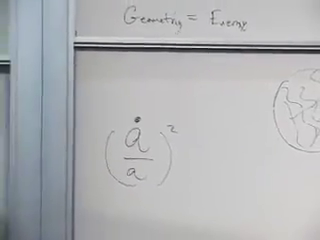
\includegraphics[width=0.68\textwidth]{lecture_06_figure_03.png}
\lectureframe{01:06:37.088}
\caption{팽창 항 \(H^2=(\dot a/a)^2\)을 그 아래에 적은, 핵심 표어 \emph{기하학은 에너지다}.}
\end{figure}

균일하고 등방적인 우주에서 제1 프리드만 방정식은 다음과 같다.
\begin{equation}
H^2+\frac{k}{a^2}
=\frac{8\pi G}{3}\rho,
\end{equation}
단위는 \(c=1\)이며, \(k=+1,0,-1\)는 닫힌 공간, 평탄한 공간, 열린 공간의 기하학을 나타낸다. 또한
\begin{equation}
\rho
=\rho_{\mathrm{ordinary}}
+\rho_{\mathrm{dark}}
+\rho_{\mathrm{radiation}}
+\rho_{\mathrm{vacuum}}.
\end{equation}
칠판에서 \(1/a^2\) 옆에 보이는 부호는 곡률 항을 좌변에 둘지 우변으로 옮길지, 그리고 \(k\)의 값이 무엇인지에 따라 달라진다.

\begin{figure}[H]
\centering
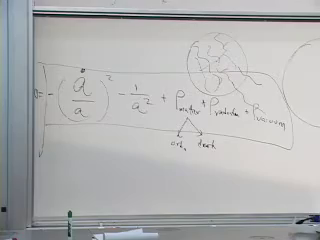
\includegraphics[width=0.96\textwidth]{lecture_06_figure_04.png}
\lectureframe{01:08:46.794}
\caption{칠판에 적힌 전체적인 균형식. 기하학 쪽에는 팽창과 공간 곡률이 있고, 원천 쪽에는 물질, 복사, 진공 에너지가 있다. 물질은 다시 보통 물질과 암흑 물질로 나뉜다.}
\end{figure}

\subsection{우주론적 해밀토니안 제약 조건}

\begin{classroomqa}
\audiencequestion{공동이동 영역 안의 진공 에너지가 우주 팽창에 따라 증가한다면, 일정한 순 에너지 밀도가 있는 것일까, 아니면 보존되는 총에너지가 있는 것일까? \lecturetimestamp{01:01:51}}
\lecturerresponse{일반 상대성 이론은 임의의 팽창 시공간에 대해 보편적인 전역 에너지를 제공하지 않는다. 그러나 균질한 우주론적 축약에서는 아인슈타인 방정식의 시간-시간 성분이 해밀토니안 제약식이다. 기하와 물질을 한쪽에 놓으면 제약된 해밀토니안은 0이 된다. 변하는 물질 항은 상자 안의 보통의 고정된 에너지가 아니라 중력 자유도에 의해 균형을 이룬다.}
\end{classroomqa}

개략적으로 쓰면 정준 관계는
\begin{equation}
\mathcal H_{\mathrm{gravity}}
+\mathcal H_{\mathrm{matter}}
=0.
\end{equation}
총에너지가 0이라고 말할 때의 정확한 의미가 이것이다. 이는 시간 재매개화 불변성이 강제하는 운동방정식이지, 모든 국소 에너지 밀도가 사라진다는 주장이 아니다. 공변 부피에서 보통 물질의 에너지는 대략 일정하고 복사 에너지는 감소하며 진공 에너지는 증가한다. 한편 중력 기여분과 팽창률은 아인슈타인 제약식이 계속 성립하도록 조정된다.

국소 보존은 여전히 정확히 성립한다:
\begin{equation}
\nabla_\mu T^{\mu\nu}=0.
\end{equation}
균일한 유체의 경우 이는 바로 연속 방정식이다.
\(\dot\rho+3H(\rho+p)=0\). 일반적으로 성립하지 않는 것은, 팽창하는 우주에서도 민코프스키 시공간에서의 직관처럼 좌표계에 무관한 전역적인 물질 에너지 총량 하나가 보존되어야 한다는 생각이다.\editorialnote{이러한 구분을 통해 에너지는 항상 0이라는 수업 중 설명을 정확히 이해할 수 있다. 국소 공변 보존 법칙과 우주론적 해밀토니안 제약식은 정확히 성립하지만, 물질과 중력을 합한 유일한 전역 에너지는 일반적으로 정의되지 않는다.}

\begin{classroomqa}\audiencequestion{에너지 제약식이 우주가 열린 우주인지, 닫힌 우주인지, 평탄한 우주인지를 결정하는 조건인가요? \lecturetimestamp{01:04:42}}\lecturerresponse{아니다. 해밀토니안 제약식은 모든 경우에 적용된다. 열린 우주, 평탄한 우주, 닫힌 우주는 곡률 표지 \(k\)에 따라, 따라서 \(k/a^2\) 항에 따라 서로 다르다. 곡률은 에너지 균형에서 한 기여 항을 바꾸지만, 제약식의 적용 여부를 바꾸지는 않는다.}\end{classroomqa}

\section{그라스만 좌표와 초장}

\begin{classroomqa}\audiencequestion{그라스만 수는 실제로 이론의 라그랑지안에 등장하나요? \lecturetimestamp{01:09:37}}\lecturerresponse{먼저 페르미온 장이 그라스만 홀수이기 때문에 등장한다. 또 초공간의 좌표로도 등장한다. 초장은 이 홀수 좌표에 의존하며, 초대칭 작용은 이 좌표에 관해 미분하고 적분하여 구성한다.}\end{classroomqa}

보통 장은 시공간의 함수다.
\begin{equation}
\phi=\phi(x^\mu).
\end{equation}
4차원 최소 초대칭에서는 \(x^\mu\)에 두 성분 홀수 스피너 \(\theta^\alpha\)와 그 켤레 \(\bar\theta^{\dot\alpha}\)를 더한다:
\begin{equation}
z^M=(x^\mu,\theta^\alpha,\bar\theta^{\dot\alpha}).
\end{equation}
복소 홀수 성분은 둘이며, 실수 홀수 방향은 넷이다. 초장은 이 초공간 위의 함수다:
\begin{equation}
\Phi=\Phi(x,\theta,\bar\theta).
\end{equation}

이것들은 계량의 의미에서 작은 공간 차원이 아니다. 그라스만 좌표에는 양의 수치적 크기가 없다. 그것이 작다고 부르는 것은 멱영성을 기억하기 위한 표현이다:
\begin{equation}
(\theta^\alpha)^2=0,
\qquad
\theta^\alpha\theta^\beta=-\theta^\beta\theta^\alpha.
\end{equation}
\editorialnote{유한 개의 그라스만 좌표에 대한 모든 전개가 끝나는 이유는 수치적으로 작아서가 아니라 멱영성이 있기 때문이다.}

서로 독립인 홀수 좌표가 넷이면, 가장 일반적인 초장은 그라스만 단항식을 최대 \(2^4=16\)개까지 포함할 수 있다. 개략적으로 쓰면
\begin{equation}
\begin{aligned}
\Phi(x,\Theta)={}&\phi(x)+\Theta_A\psi_A(x)\\
&+\frac{1}{2}\Theta_A\Theta_B Z_{AB}(x)+\cdots\\
&+\Theta_1\Theta_2\Theta_3\Theta_4D(x),
\end{aligned}
\end{equation}
여기서 \(\Theta_A\)는 네 실수 홀수 좌표를 통칭한다. 초장 전체를 짝수로 택할 수 있으므로, 짝수 차수 항의 계수는 보손이고 홀수 차수 항의 계수는 페르미온이다. 따라서 초장 하나에 보통 성분장들로 이루어진 유한한 다중항이 담긴다.

이러한 묶음은 단순한 표기상의 편의 이상이다. 초대칭은 시공간 병진과 뒤섞인 홀수 방향의 병진으로 기하학적으로 작용한다. 텐서로 구성한 스칼라 라그랑지안이 회전 또는 로런츠 불변성을 따르듯, 초공간 규칙에 따라 초장으로 구성한 라그랑지안은 초대칭을 물려받는다.

이제 작용에는 그라스만 측도가 포함된다. 전형적인 전체 초공간 항은 다음과 같다.
\begin{equation}
S_D=\int d^4x\,d^2\theta\,d^2\bar\theta\,
\mathcal K(\Phi,\Phi^\dagger).
\end{equation}
반면 카이럴 항에는 다음 측도를 쓴다.
\begin{equation}
S_F=\int d^4x\,d^2\theta\,W(\Phi)+\mathrm{h.c.}
\end{equation}
\editorialnote{전체 초공간 측도와 카이럴 측도의 구분은 개략적인 \(d^4x\,d^4\theta\) 작용을 표준적인 방식으로 세분한 것이다. 어떤 측도가 적절한지는 구체적인 예를 통해 정해진다.}

따라서 이제 보통 미적분학으로는 답할 수 없는 질문에 이르렀다. 반가환 좌표에 대한 적분은 무엇을 뜻하는가?

\section{베레진 적분}

\subsection{보통의 본보기: 전미분}

보통 함수 \(F(x)\)부터 시작하자. 이 함수는 큰 양수와 큰 음수의 \(x\)에서 함수값이 사라진다. 미적분학의 기본 정리에 따르면
\begin{equation}
\int_{-\infty}^{\infty}dx\,\frac{dF}{dx}
=F(\infty)-F(-\infty)
=0.
\end{equation}

\begin{figure}[H]
\centering
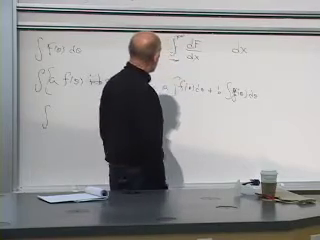
\includegraphics[width=0.88\textwidth]{lecture_06_figure_05.png}
\lectureframe{01:26:31.594}
\caption{베레진 적분의 일반적인 원형은 전체 도함수의 적분이 경계값으로 환원되며 함수가 충분히 빠르게 감쇠하면 적분값도 사라진다는 것이다. 아래쪽 칠판 줄은 일부 가려져 있어 본문에 식을 옮겨 적었다.}
\end{figure}

그라스만 적분이 선형이고 전미분의 적분이 0이 되는 유용한 성질을 공유하도록 하자. 홀수 좌표 하나에 대해서는 다음을 요구한다.
\begin{align}
\int d\theta\,[af(\theta)+bg(\theta)]
&=
a\int d\theta\,f(\theta)
+b\int d\theta\,g(\theta),\\
\int d\theta\,\partial_\theta f(\theta)&=0.
\end{align}
두 번째 조건은 측도의 병진 불변성에 해당하는 대수적 조건이다. 홀수 수직선에는 끝점이 없으며, 작은 구간에 대한 합도 없다.

\begin{classroomqa}\audiencequestion{부정 그라스만 적분이 없다면, 적분이 미분의 역연산이라는 생각을 포기하는 건가요? \lecturetimestamp{01:21:19}}\lecturerresponse{그렇다. 베레진 적분은 원시함수 연산이 아니라 정적분을 주는 선형 함수다. 그라스만 변수 하나의 경우에는 실제로 미분과 같은 대수적 연산으로 나타난다.}\end{classroomqa}

\begin{classroomqa}\audiencequestion{시공간 전체에 대한 \(d^4x\) 적분도 정적분인가요? \lecturetimestamp{01:21:34}}\lecturerresponse{그렇다. 작용을 시공간에 대해 적분할 때는 경계 조건을 전제한다. 차이는 보통 시공간 적분은 합의 극한으로 이해할 수 있는 반면, 그라스만 적분은 유한한 기저 \(1,\theta\)에 작용하는 방식으로 대수적으로 정의된다는 점이다.}\end{classroomqa}

\subsection{변수 하나}

홀수 변수 하나의 모든 함수는 계수를 정해진 오른쪽 순서로 놓아 다음과 같이 쓸 수 있다.
\begin{equation}
f(\theta)=a+\theta b.
\end{equation}
\(\partial_\theta\theta=1\)이므로, 전미분 규칙에 따라 다음을 얻는다.
\begin{equation}
\int d\theta\,1=0.
\end{equation}
나머지 정규화는 다음과 같이 정한다.
\begin{equation}
\int d\theta\,\theta=1.
\end{equation}
따라서
\begin{equation}
\int d\theta\,f(\theta)=b.
\end{equation}
적분은 가능한 최고 차수 항의 계수를 추출한다. 여기서 사용하는 좌미분 규약에서는
\begin{equation}
\partial_\theta f=b
=\int d\theta\,f.
\end{equation}

\begin{classroomqa}\audiencequestion{조건 \(\partial_\theta F=\theta\)을 만족하는 함수 \(F(\theta)\)가 있나요? \lecturetimestamp{01:30:05}}\lecturerresponse{없다. 그런 함수에는 \(\theta^2\)에 비례하는 항이 있어야 하지만 \(\theta^2=0\). 이는 그라스만 변수에서 부정 적분에 해당하는 것이 없는 이유를 보여주는 또 다른 방식이다.}\end{classroomqa}

\subsection{변수 두 개와 적분 측도의 순서}

복소 변수 쌍 \(\theta,\bar\theta\)에 대해 일반적인 짝수 함수를 정해진 순서로 쓰면 다음과 같다.
\begin{equation}
f(\theta,\bar\theta)
=a+\bar\theta\psi+\bar\psi\theta+b\,\bar\theta\theta.
\end{equation}
\begin{equation}
\theta^2=\bar\theta^2=0,
\qquad
\bar\theta\theta=-\theta\bar\theta.
\end{equation}이므로 더 높은 차수 항은 없다.

이제 다음 규약을 정한다.
\begin{equation}
\int d\theta\,d\bar\theta\,
\bar\theta\theta=1.
\end{equation}
반복 적분에서는 인접한 \(d\bar\theta\) 연산이 먼저 작용한다. 그러면 표는 다음과 같다.
\begin{align}
\int d\theta\,d\bar\theta\,1&=0,\\
\int d\theta\,d\bar\theta\,\theta&=0,\\
\int d\theta\,d\bar\theta\,\bar\theta&=0,\\
\int d\theta\,d\bar\theta\,\bar\theta\theta&=1.
\end{align}
따라서
\begin{equation}
\int d\theta\,d\bar\theta\,
f(\theta,\bar\theta)=b.
\end{equation}

\begin{classroomqa}
\audiencequestion{\(\theta\)에 선형인 항에서는 이중 적분을 사라지게 하는 것이 정말 \(\theta\) 적분인가요?\lecturetimestamp{01:34:59}}
\lecturerresponse{아니다. 강의 중 설명에서 두 적분의 역할이 뒤바뀌어 있었다. \(\theta\)를 \(\theta\)에 대해 적분하면 1이 된다. 그러면 결과에는 더 이상 \(\bar\theta\)가 없고, 남은 \(\bar\theta\)에 대한 적분은 1을 적분하므로 사라진다. 어느 경우든 두 변수가 모두 들어 있어야 이중 적분이 살아남는다.}
\end{classroomqa}

\begin{classroomqa}\audiencequestion{\(\theta\)와 \(\bar\theta\)의 순서를 바꾸면 적분의 부호가 바뀌나요? \lecturetimestamp{01:36:33}}\lecturerresponse{그렇다. 홀수 변수와 홀수 측도는 서로 반가환한다. 위에서 정한 규약에서는
\[
\int d\bar\theta\,d\theta\,\bar\theta\theta=-1.
\]
따라서 순서를 하나 정해 일관되게 유지해야 한다. 물리는 규약에 무관하지만 중간 계산의 부호는 그렇지 않다.}\end{classroomqa}

서로 독립인 그라스만 변수가 \(n\)개일 때는 규칙을 바로 일반화할 수 있다.
\begin{equation}
\int d\theta_n\cdots d\theta_1\,
f(\theta_1,\ldots,\theta_n)
\end{equation}
이 적분은 변수와 측도에 대해 선택한 순서로 정해지는 부호까지 고려하면, 정렬된 최고차 단항식 \(\theta_1\cdots\theta_n\)의 계수를 추출한다. 이 간단한 성분 추출 규칙이 초공간 작용의 핵심이다. 초대칭 변분은 홀수 전미분이 되고, 초공간 적분은 이를 제거한다. 적절한 경계 조건 아래 보통 작용이 시공간 전미분을 제거하는 것과 같다.

\section{이처럼 단순한 계산법이 강력한 이유}

규칙은 거의 자명해 보인다:
\begin{equation}
\int d\theta\,1=0,
\qquad
\int d\theta\,\theta=1.
\end{equation}
그럼에도 이 규칙으로 보손과 페르미온의 질량 및 결합 상수 사이의 관계가 자동으로 유지되는 상호작용 장론을 구성할 수 있다. 초공간 계산법의 목적은 상대론에서 텐서 계산법의 목적과 같다. 허용된 모든 조작을 거쳐도 원하는 대칭성이 유지되도록 표기를 구성하는 것이다.

그 대가로 부호를 꼼꼼히 따져야 한다. 홀수인 두 대상을 맞바꿀 때마다 마이너스 부호가 생기며, 개념적으로는 옳은 계산도 순서를 한 번 잘못 정하면 틀릴 수 있다. 이 어려움은 장식적인 것이 아니라 페르미온 통계가 대수에 드리우는 흔적이다.

\begin{classroomqa}\audiencequestion{그라스만 수는 초대칭과 함께 발명되었나요, 아니면 더 일찍 등장했나요? \lecturetimestamp{01:41:19}}\lecturerresponse{그라스만 수는 훨씬 오래되었다. 헤르만 그라스만은 19세기에 그 기초가 되는 외대수를 발전시켰다. 미분형식에는 이미 반가환 기저 원소가 쓰인다. 20세기 양자장론과 초대칭은 같은 수학에서 새로운 물리적 역할을 발견했다.}\end{classroomqa}

이제 구체적인 구성을 살펴볼 준비가 되었다. 초장은 보손과 페르미온으로 이루어진 완전한 다중항을 담고, 초공간 미분은 대수 구조를 보존하며, 베레진 적분은 성분 작용을 추출한다. 다음으로 이 도구를 가장 단순한 1차원 모형에 적용한 뒤 장론으로 확장한다.
